\documentclass{bmvc2k}

%% Enter your paper number here for the review copyu
\bmvcreviewcopy{666}

\title{Correspondence matching of non-coplanar circles from a single image}

% Enter the paper's authors in order
% \addauthor{Name}{email/homepage}{INSTITUTION_CODE}
\addauthor{Susan Student}{http://www.vision.inst.ac.uk/~ss}{1}
\addauthor{Petra Prof}{http://www.vision.inst.ac.uk/~pp}{1}
\addauthor{Colin Collaborator}{colin@collaborators.com}{2}

% Enter the institutions
% \addinstitution{Name\\Address}
\addinstitution{
 The Vision Institute\\
 University of Borsetshire\\
 Wimbleham, UK
}
\addinstitution{
 Collaborators, Inc.\\
 123 Park Avenue,\\
 New York, USA
}

\runninghead{Student, Prof, Collaborator}{BMVC Author Guidelines}

% Any macro definitions you would like to include
% These are not defined in the style file, because they don't begin
% with \bmva, so they might conflict with the user's own macros.
% The \bmvaOneDot macro adds a full stop unless there is one in the
% text already.
\def\eg{\emph{e.g}\bmvaOneDot}
\def\Eg{\emph{E.g}\bmvaOneDot}
\def\etal{\emph{et al}\bmvaOneDot}

%------------------------------------------------------------------------- 
% Document starts here
\begin{document}

\maketitle

\begin{abstract}
In this work we have proposed a method to determine 2D-3D correspondence between non-coplanar circles from a single image.
Our method uses image conics to compute circle plane orientation in camera coordinate system, thus bringing the problem from 2D to 3D domain. This information is used to generate projective invariant descriptors which can be used directly for correspondence matching, given that the 3D information about circles are known. Additionally, the evaluation also covers study stability of the projective invariants and the factors affecting their computation. One of the intended applications is for tracking industrial objects with circles on it. In our approach we use conic properties of circles to compute projective invariant descriptors. These descriptors are matched with known 3D information to establish correspondences. We also demonstrate stability of the invariants used to generate descriptors,   
In our approach we compute 3D plane orientation of each circle from its image contour, and compute projective invariants between each pair of circles. We propose a new descriptor 

\end{abstract}

%------------------------------------------------------------------------- 
\section{Introduction}
\label{sec:intro}
Correspondence matching is one of the key problems in computer vision. Applications related to pose estimation or object detection require accurate knowledge of model features and their corresponding image features. This is a challenging problem especially for monocular systems. Machine learning based methods \cite{Hartley00} provide promising results, but are limited to a specific group of objects and require prior learning of the object. Many authors have proposed using natural features like points, lines and conics for solving correspondence problem. The core idea is to compute projective invariants from such features to obtain robust matching with model feature points.[Quan] One approach is using two or more images from different perspective to find same image features and then obtain correspondence using triangulation technique. The problem is more complex with a single image as depth feature is lost. In this paper we will focus on solving this particular problem of matching from a single image. 

Using points and lines to establish correspondence is 

Explain the problem in question, the motivation for the work and the proposed application in mind.
No much work done in this direction. The invariants proposed are never used for a application so we provide use and discuss stability of the algorithm. Comment on why circles and the paper we build up to. 
The work of Forsyth as the base of our work, the concepts given in the paper. Our contribution is matching strategy using such invariants. Demonstrating an application and evaluation of the method. 

The assumptions made in our work. We have the camera calibrated and we use 3D points and their normal positions for the descriptor measurement. 

%-> Figure explaining the issue 
%\begin{figure}
%\begin{tabular}{ccc}
%\bmvaHangBox{\fbox{\parbox{2.7cm}{~\\[2.8mm]
%\rule{0pt}{1ex}\hspace{2.24mm}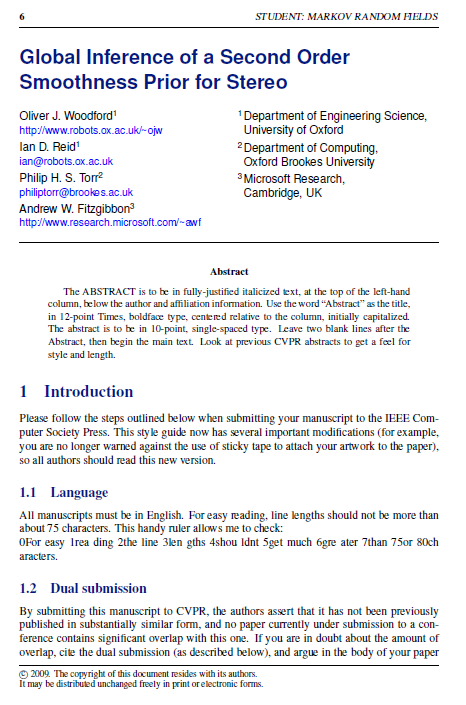
\includegraphics[width=2.33cm]{images/eg1_largeprint.png}\\[-0.1pt]}}}&
%\bmvaHangBox{\fbox{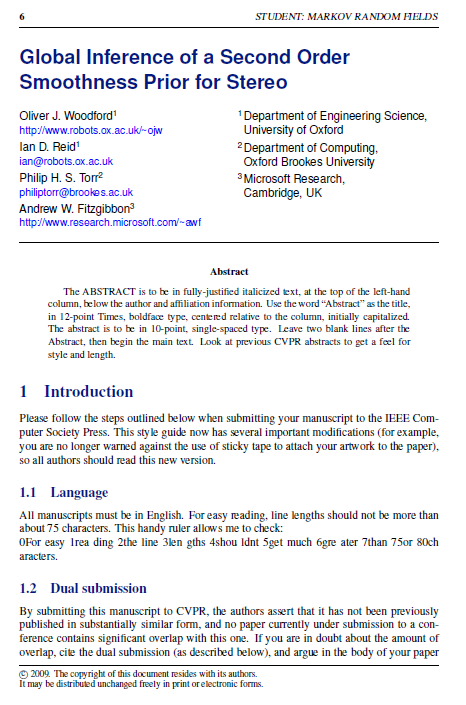
\includegraphics[width=2.8cm]{images/eg1_largeprint.png}}}&
%\bmvaHangBox{\fbox{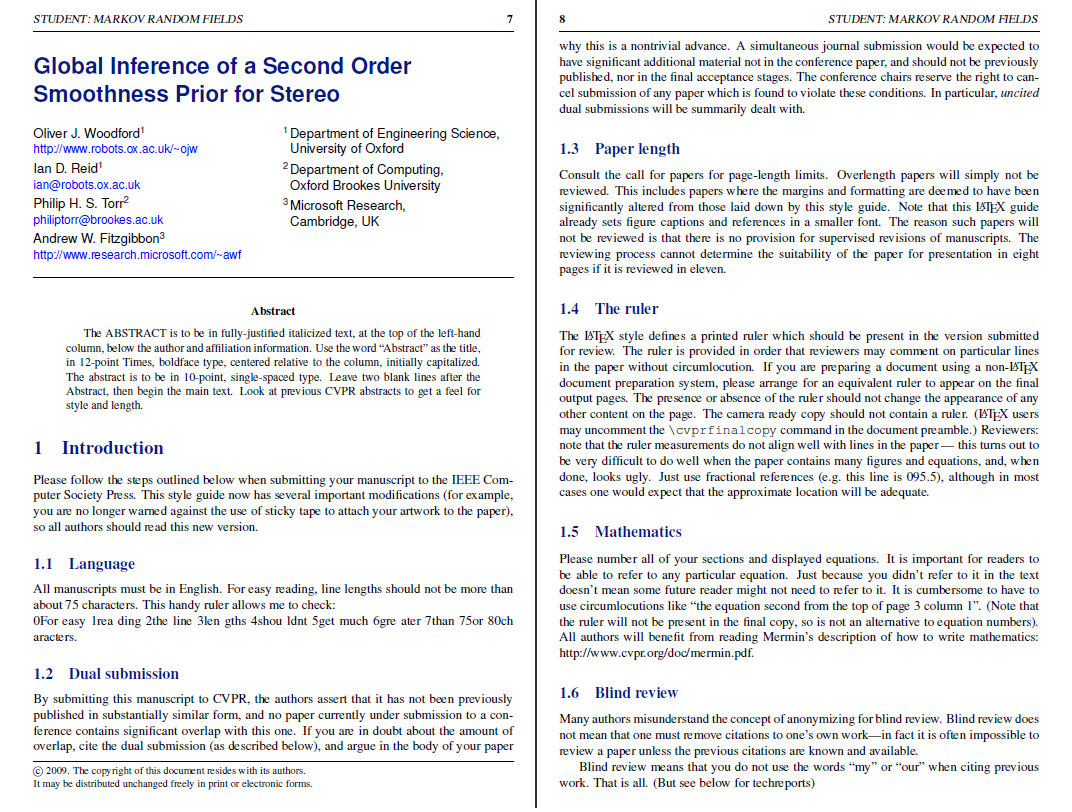
\includegraphics[width=5.6cm]{images/eg1_2up.png}}}\\
%(a)&(b)&(c)
%\end{tabular}
%\caption{It is often a good idea for the first figure to attempt to
%encapsulate the article, complementing the abstract.  This figure illustrates
%the various print and on-screen layouts for which this paper format has
%been optimized: (a) traditional BMVC print format; (b) on-screen
%single-column format, or large-print paper; (c) full-screen two column, or
%2-up printing. }
%\label{fig:teaser}
%\end{figure}



\section{Related Work}

Many applications in vision or augmented reality using points and lines for single image correspondence. 
Work done by zissermann and safreed on computing 3D position. Single circle based coded solution proposed by TRIP. 
We work on problem of un-coded circles which can very much be natural features of a particular model.  

We are fixed on fiducial based systems or sparce points and therefore other solutions of markerless are not idea because selection of feature points in not in users hand.

Write about the uniquness of the work and proposed analysis of the invariants. 

\section{Method}
Page 3: 
The available information as input (3D points and normals), the concept of descriptor and back ground of the re-projection 
A simple input and output function that explains the process in nutshell. 
\subsection{Invariants}
The invariants generated by a pair of circles. 
The computation of plane orientation from image contour. 
The ambiguity is explained and complexity added due to ambiguity is explained. 
\subsection{Descriptor design}
The simulations done for the invariants are commented and comments are made on 
A descriptor represents two unique points and not one point. Unlike many methods used these days. 
<d,theta>, <d,th1,th12,th21,th22>. 
Since both are not exactly same a matching strategy is developed to have point to point correspondence.    
\subsection{Step 1: Initial Pairwise Matching}
- Algorithm (Select pairs as tentitive matches by matching d and theta with some threshold)
- Explain the pairwise matching 
%------------------------------------------------------------------------- 
\subsection{Step 2: Triplet Matching}
Why? : because of ambiguity lot of results are false, by adding another constraint we restrict the probability of false matching. Also to make it point wise problem from a pair wise problem. 
- Matching steps on voting 
- Solving problem from pairwise matching to point wise matching
\subsection{Step 3: Hypothesis generation}
Filter the voting matrix to generate point wise matching hypothesis. 
Comment on how many would be enough to check other hypothesis. 
(3 are enough to predict solutions) since we know the calibration. 
One can select only top voted 3 pairs (since they are 3D points) and then verify the whole choice, or go for 6 point matching and achieve the same.

%\begin{figure*}
%\begin{center}
%\fbox{\rule{0pt}{2in} \rule{.9\linewidth}{0pt}}
%\end{center}
%   \caption{Example of a short caption, which should be centered.}
%\label{fig:short}
%\end{figure*}

%\begin{table}
%\begin{center}
%\begin{tabular}{|l|c|}
%\hline
%Method & Frobnability \\
%\hline\hline
%Theirs & Frumpy \\
%Yours & Frobbly \\
%Ours & Makes one's heart Frob\\
%\hline
%\end{tabular}
%\end{center}
%\caption{Results.   Ours is better.}
%\end{table}

\section{Evaluation}
Page 5: 
Explain the experiment models. The selection of the markers as per standard. 
Model 1 : 12mm 
Model 2 : 8mm-5mm 
Ground truth : GOM data for 3D information and ground truth for 3D and 2D correspondences. 
%------------------------------------------------------------------------- 
\subsection{Matching comparison}
1. Exp 1 : Models in the frame with different pose 
Comment : How are images taken, Fixed camera distances 
Table : No of input points , No of Matched points , No of correct Match, No of Images
1. For model 12 mm 
2. For model 5 mm

2. Exp 2 : Models in presence of each other (False positive rejection (on and off the model) )
How are images taken, which model is supposed to be tracked, Addition of false positives in the scene. 
1. 12mm car with 8mm/5mm car model 

2. 8 mm with 5mm on itself (Bad results) : Is this experiment important? or Experiment with other model with 12 mm configuration. (Bad matching results removed by voting filtering). 

3. 12 mm with 130 false positives and computing the right model. 
%------------------------------------------------------------------------
\subsection{Time}
Time taken for high resolution images and low resolution images. Tracking applications specific performance comments. Suitable for real time applications like in AR. 

\section{Conclusion}
Page 7 : 
1. Reliable method for correspondence matching for non coplananr circular features. 
2. Accuracy is improved with the size and method works better if the detection range is selected appropriate to the conic size. 
3. Comment on the stability of the invariants 

\section{Future Applications}
Future work : 
1. 2D-2D correspondence to triangulate from multiple images to get rid of the initial condition. 
2. Improving the matching method for higher runtime performance.
3. Using normals obtained for solving p3p problem. 

Each model has its own orientation and random arrangement gives us choice between tracking same models with individual identity. 


\bibliography{egbib}
\end{document}
